\section{Fact Extraction}
\label{sec:stage1}
% ============================================================

The initial input to the synthesis pipeline is a paragraph of natural-language prose ($\mathcal{D}$). Fact Extraction transforms $\mathcal{D}$ into a set of discrete, \emph{atomic facts} ($\mathcal{F}$). By decomposing the text, removing ambiguities, and resolving information deficiencies through targeted enrichment, this stage ensures the domain is rigorously defined before any structural modelling begins. Furthermore, extracting requirements as atomic units provides strict provenance, enabling every subsequent schema decision to be traced directly back to the specific evidence that justified it.

\subsection{Atomic Extraction and Verification}
\label{subsec:extraction}

\begin{figure}[t]
  \centering
  % If the space in the filename impedes compilation, rename the PDF to a space-free name.
  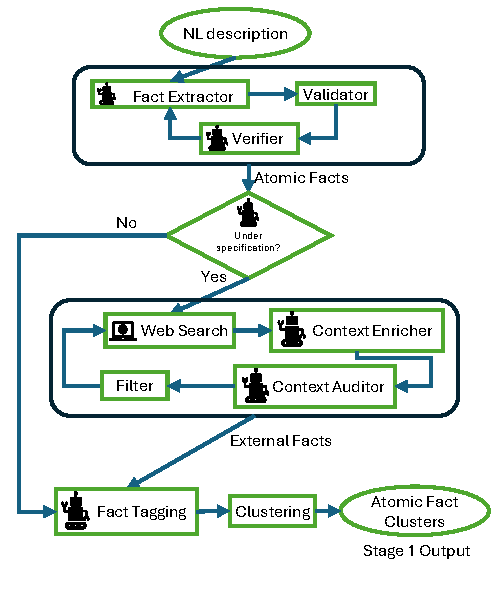
\includegraphics[width=\columnwidth,page=1]{ScribbleDB Image.pdf}
  \caption{The Fact Extraction stage. A verified set of atomic facts is gated on
  completeness; under-specified inputs are enriched against retrieved web evidence under a
  semantic auditor and a deterministic structural filter before all facts are tagged and
  clustered. The stage emits clusters of atomic facts, the sole input to Schema
  Generation (\S\ref{sec:stage2}).}
  \label{fig:stage1}
\end{figure}

An atomic fact encapsulates exactly one requirement: the existence of an entity, a specific attribute, a relationship, or a logical rule. For example, the statement ``An applicant has a credit score between 300 and 850'' is decomposed into two distinct facts: (1) an applicant has a credit score, and (2) a credit score lies between 300 and 850. This strict atomicity decouples structural definitions from logical constraints.

To ensure traceability, every fact is anchored to the specific span of $\mathcal{D}$ that justifies it. Instead of relying on an LLM to unreliably output character offsets, the extractor returns an ordered list of verbatim substrings from $\mathcal{D}$, with the atomic facts nested beneath them. Precise character offsets are then recovered via a deterministic scan.

Because initial extraction requires semantic judgement, it is delegated to an LLM agent. However, to guarantee fidelity, the output is iteratively scrutinized by a localized \emph{Dual Guard} repair loop (Figure~\ref{fig:stage1}, top). The first guard is a deterministic \textsc{Validator} that enforces structural integrity by confirming that each fact's origin segment is genuinely a verbatim substring of $\mathcal{D}$. The second guard is an LLM-based \textsc{Verifier} that identifies semantic omissions or hallucinated details. The extractor edits only the faulted facts until the audit returns clean or a retry budget is exhausted.

\subsection{Gap-Directed Context Enrichment}
\label{subsec:enrichment}

Even a fact set that is perfectly faithful to $\mathcal{D}$ may be too sparse to induce a usable schema, as initial descriptions routinely omit foundational domain knowledge. A completeness agent evaluates the verified facts against the expected structural skeleton for the target domain. If it detects severe omissions (e.g., missing core entities), it emits typed \emph{coverage gaps} and routes the facts into an enrichment loop (Figure~\ref{fig:stage1}, center).

Enrichment augments the dataset with external facts, introducing a risk of hallucination. To mitigate this, a \textsc{Web Search} module retrieves external evidence and populates a shared pool with stable citation tags. A \textsc{ContextEnricher} proposes new facts by citing these tags. A semantic \textsc{ContextAuditor} dynamically checks every proposed fact against the retrieved text, immediately rejecting any that are ungrounded. Finally, a deterministic filter ensures the new facts anchor cleanly to the original description. The loop terminates once all severe gaps are closed and the fact set is structurally sound.

\subsection{Tagging and Fact Clustering}
\label{subsec:cluster}

The verified and enriched facts are first classified by a \textsc{Tagger} into four categories: \textsc{structural} (entities/attributes), \textsc{logical} (rules), \textsc{statistical} (distributions), and \textsc{metadata}. These tags route facts to the appropriate downstream stages.

To enable parallel schema generation, the comprehensive fact set must then be partitioned into independent groups. Rather than invoking an LLM, the partitioning is achieved mechanically by treating the provenance segments recovered during initial extraction as indivisible atomic units (Algorithm~\ref{alg:cluster}). By grouping facts mechanically based on their origin, the system preserves the local context intended by the original author.

The algorithm frames clustering as a Dirichlet Process Mixture Model driven by three complementary signals: \emph{positional adjacency} (segments close together in the text), \emph{semantic similarity} (embedding proximity), and \emph{cross-references} (explicit structural hints). Using a collapsed Gibbs sampler, the algorithm auto-calibrates the relative weights of these signals and extracts stable clusters from the consensus of posterior samples, ensuring robust partitions that serve as the definitive output of the stage.

\begin{algorithm}[t]
\caption{Segment-Grounded Fact Clustering}
\label{alg:cluster}
\begin{algorithmic}[1]
  \Require Atomic facts $\mathcal{F}$ anchored by provenance, Sampling iterations $N$
  \Ensure Disjoint fact clusters (shards) $\mathcal{C}$
  \State \textbf{Phase 1: Feature Extraction}
  \State Group $\mathcal{F}$ into indivisible text segments based on their character positions in the source document
  \State $\mathbf{S}_{\text{sim}} \gets$ Compute semantic similarity matrix using text embeddings of the segments
  \State $\mathbf{S}_{\text{adj}} \gets$ Compute positional proximity matrix ($1 / (1 + \text{text\_distance})$)
  \State $\mathbf{R} \gets$ Extract binary matrix of explicit cross-references between segments
  
  \State \textbf{Phase 2: Iterative Cluster Refinement (Gibbs Sampling)}
  \State Initialize each segment into its own isolated cluster
  \For{iteration $t = 1$ \textbf{to} $N$}
    \State $\mathbf{W} \gets$ Dynamically fuse $\mathbf{S}_{\text{adj}}$ and $\mathbf{S}_{\text{sim}}$ using auto-tuned mixing weight $\lambda$
    \For{each segment $i$ in a randomized order}
      \State Temporarily remove $i$ from its current cluster
      \State \textbf{for} each active cluster $k$, calculate affinity score based on:
      \State \quad - The structural density of $\mathbf{W}$ between $i$ and all members of $k$
      \State \quad - A strong reward for any direct cross-references $\mathbf{R}$ with members of $k$
      \State Calculate the baseline penalty for isolating $i$ into a newly formed cluster
      \State Probabilistically reassign $i$ to a cluster based on normalized affinity scores
    \EndFor
    \If{$t$ is a calibration interval}
      \State Re-calibrate $\lambda$ and internal affinity parameters based on current cluster densities
    \EndIf
    \State Record segment co-occurrences for this iteration (post-burn-in)
  \EndFor
  
  \State \textbf{Phase 3: Consensus Extraction}
  \State $\mathbf{M} \gets$ Build co-association matrix (frequency of segments sharing a cluster across all iterations)
  \State Partition $\mathbf{M}$ at a 50\% consensus threshold to finalize stable segment clusters
  \State $\mathcal{C} \gets$ Map the grouped segments back to their constituent atomic facts $\subset \mathcal{F}$
  \State \Return $\mathcal{C}$
\end{algorithmic}
\end{algorithm}
